% !TEX program = xelatex
\documentclass[UTF8,fontset=fandol,a4paper,11pt]{ctexart}
\usepackage[margin=21mm,top=23mm,bottom=22mm,headheight=16pt]{geometry}
\usepackage{amsmath,amssymb,mathtools,bm}
\usepackage{tikz}
\usetikzlibrary{arrows.meta,calc,angles,quotes,patterns,decorations.pathmorphing}
\usepackage{xcolor,booktabs,array,longtable,enumitem,fancyhdr,needspace}
\usepackage[unicode,hidelinks]{hyperref}
\definecolor{ink}{HTML}{24343C}
\definecolor{accent}{HTML}{166A70}
\definecolor{muted}{HTML}{65747A}
\definecolor{rulegray}{HTML}{D4DDE0}
\definecolor{warm}{HTML}{966037}
\color{ink}
\setlength{\parindent}{2em}
\setlength{\parskip}{4pt}
\linespread{1.12}
\AtBeginDocument{\setlength{\abovedisplayskip}{6pt plus 2pt minus 1pt}
\setlength{\belowdisplayskip}{6pt plus 2pt minus 1pt}
\setlength{\abovedisplayshortskip}{0pt plus 1pt}
\setlength{\belowdisplayshortskip}{4pt plus 1pt}}
\setlist[enumerate]{label=(\arabic*),leftmargin=2.3em,itemsep=3pt,topsep=4pt}
\setlist[itemize]{leftmargin=2em,itemsep=2pt,topsep=4pt}
\allowdisplaybreaks[1]
\setlength{\emergencystretch}{2em}
\setcounter{secnumdepth}{0}
\providecommand{\tightlist}{\setlength{\itemsep}{0pt}\setlength{\parskip}{0pt}}
\ctexset{section={format=\Large\bfseries\color{accent},beforeskip=10pt,afterskip=9pt},
subsection={format=\normalsize\bfseries\color{accent},beforeskip=10pt,afterskip=4pt},
subsubsection={format=\normalsize\bfseries,beforeskip=8pt,afterskip=3pt}}
\pagestyle{fancy}
\fancyhf{}
\fancyhead[L]{\small\color{muted}物理学难题集萃}
% 页眉仅保留书名；版本名称只在封面显示。
\fancyfoot[L]{\small\color{muted}\chapterlabel}
\fancyfoot[R]{\small\thepage}
\renewcommand{\headrulewidth}{0.4pt}
\renewcommand{\footrulewidth}{0pt}
\newcommand{\dd}{\mathop{}\!\mathrm{d}}
\newcommand{\vect}[1]{\bm{#1}}
\newcommand{\tagline}[1]{\noindent{\small\color{muted}#1}\par}
\newcommand{\result}[1]{\begin{equation*}\boxed{#1}\end{equation*}}
\newcommand{\figcaption}[1]{\par\vspace{2pt}{\small\color{muted}#1}\par}
\newcommand{\teach}[2]{\Needspace{4\baselineskip}\subsection*{讲解要点与追问}#1\par\smallskip\noindent\textbf{追问：}#2\par}
\newcommand{\workarea}{\par\vspace{7mm}\noindent{\small\color{muted}作答区}\par\vspace{4mm}
\noindent\textcolor{rulegray}{\rule{\linewidth}{0.3pt}}\par\vspace{16mm}
\noindent\textcolor{rulegray}{\rule{\linewidth}{0.3pt}}\par\vspace{16mm}
\noindent\textcolor{rulegray}{\rule{\linewidth}{0.3pt}}\par\vspace{16mm}
\noindent\textcolor{rulegray}{\rule{\linewidth}{0.3pt}}}
\tikzset{axis/.style={-{Stealth[length=2mm]},thin,color=muted},
motion/.style={-{Stealth[length=2.3mm]},thick,color=accent},
force/.style={-{Stealth[length=2.3mm]},thick,color=warm},
traj/.style={thick,color=accent},guide/.style={dashed,thin,color=muted},
object/.style={thick,color=ink},every node/.style={font=\small}}\renewcommand{\result}[1]{\boxed{#1}}\widowpenalty=10000\clubpenalty=10000\displaywidowpenalty=10000

\newcommand{\chapterlabel}{第六章\quad 刚体动力学}
\hypersetup{pdftitle={第六章 刚体动力学·学生版},pdfauthor={},pdfsubject={第六章第1--27题}}
\begin{document}
\pdfbookmark[0]{第六章 刚体动力学}{cover}
\thispagestyle{empty}
\vspace*{20mm}
\noindent{\Huge\bfseries 物理学难题集萃}\par\vspace{8mm}
\noindent{\LARGE 第六章\quad 刚体动力学}\par\vspace{10mm}
\noindent{\Large\color{accent}学生版}\par\vspace{8mm}
\noindent\textcolor{accent}{\rule{\linewidth}{1pt}}\par\vspace{8mm}
\noindent 第 1--27 题\par\vspace{5mm}
\noindent 题目、题图与作答区。\par
\vfill\clearpage
\pdfbookmark[1]{题目目录}{contents}
\section*{题目目录}
\begin{longtable}{@{}>{\color{accent}\bfseries}r p{120mm}@{}}
\toprule 题号 & 题目\\\midrule
1 & 汽车后轮驱动不打滑的摩擦条件 \\
2 & 均匀圆柱体绕斜向质心轴的转动惯量 \\
3 & 桌边细杆开始滑动的临界角 \\
4 & 实心圆柱体绕桌边下滚与开始滑动 \\
5 & 甲虫落到可转动麦杆后的运动 \\
6 & 圆柱滚上台阶的速度范围 \\
7 & 地月系统角动量与月球退行 \\
8 & 行星自转与卫星圆轨道的角动量转移 \\
9 & 线轴受拉时的滚动方向与加速度 \\
10 & 斜面木块牵引实心圆柱体的滚动动力学 \\
11 & 逆向自旋乒乓球由滚滑转为纯滚 \\
12 & 圆柱体滚下斜坡撞墙后的回升高度 \\
13 & 小球沿圆柱面滚下的无滑条件 \\
14 & 两相同实心球弹性碰撞后的滚动 \\
15 & 两圆柱轮与轻杆连接系统的运动 \\
16 & 带初始自旋实心球碰地后的反弹 \\
17 & 圆柱体在可动斜面上无滑滚动 \\
18 & 实心球在水平面内的滚滑运动 \\
19 & 两均匀圆盘偏心碰撞后的速度与转动 \\
20 & 细圆环在粗糙桌面上的滑动与转动衰减 \\
21 & 竖直均匀细杆在光滑地面上倒下 \\
22 & 质点撞击光滑地面上均匀细杆 \\
23 & 细杆靠墙下滑的运动与离墙 \\
24 & 单杆与铰接双段杆受相同冲量的动能比较 \\
25 & 旋转圆环中滑动细杆的平衡与稳定性 \\
26 & 旋转支架上细杆的有效势能与平衡 \\
27 & 陀螺进动与翻转陀螺的摩擦力矩机制 \\
\bottomrule\end{longtable}


\clearpage

\pdfbookmark[2]{第 1 题 汽车后轮驱动不打滑的摩擦条件}{q1}

\section*{第 1 题\quad 汽车后轮驱动不打滑的摩擦条件}

\tagline{M-06-01}

汽车在后轮的推动下,以加速度 \(a\)
在地面上沿直线前进.已知汽车前轮与后轮的间距为
\(2l\),质心位于前后轮的中央,离地高度为 \(h\),后轮与地面之间的摩擦系数为
\(\mu\),前轮为非驱动轮,与地面的摩擦可略.试问:\(\mu\)
至少为多大时,后轮不致打滑?

\begin{center}\begin{minipage}{\linewidth}\centering
\begin{tikzpicture}[font=\small]
\draw[object](-.4,0)--(5,0);\draw[object](.2,.5)rectangle(4.5,1.8);\foreach \x in {.8,3.9}{\draw[object](\x,.5)circle(.5);}\fill(2.35,1.15)circle(2pt)node[above]{$C$};\draw[guide](2.35,0)--(2.35,1.15);\node[right]at(2.35,.5){$h$};\draw[<->](.8,-.5)--(3.9,-.5)node[midway,below]{$2l$};\draw[motion](4.9,1)--(6.1,1)node[right]{$a$};\node[above]at(.8,2){后轮};\node[above]at(3.9,2){前轮};
\end{tikzpicture}
\figcaption{图 6.1\quad 后轮驱动；质心在轮距中点上方。}
\end{minipage}\end{center}

\workarea

\clearpage

\pdfbookmark[2]{第 2 题 均匀圆柱体绕斜向质心轴的转动惯量}{q2}

\section*{第 2 题\quad 均匀圆柱体绕斜向质心轴的转动惯量}

\tagline{M-06-02}

如图6.2,质量为\(m\)的均匀圆柱体,截面半径为\(R\),长为\(2R\).试求:圆柱体绕通过质心及两底面边缘的转轴(图6.2中的\(\sigma_{1}\)或\(\sigma_{2}\))的转动惯量.

\begin{center}\begin{minipage}{\linewidth}\centering
\begin{tikzpicture}[font=\small]
\draw[object](-1.5,-1.5)rectangle(1.5,1.5);
\draw[axis](-2.4,0)--(2.5,0)node[right]{$\sigma_3$};
\draw[axis](0,-2.15)--(0,2.15)node[above]{$\sigma_4$};
\draw[axis](-2,-2)--(2,2)node[above right]{$\sigma_1$};
\draw[axis](-2,2)--(2,-2)node[below right]{$\sigma_2$};
\fill(0,0)circle(1.7pt);\node at(.35,-.65){$O$};
\draw[<->](-1.5,-2.65)--(1.5,-2.65)node[midway,below]{$2R$};
\draw[<->](-2.55,0)--(-2.55,1.5)node[midway,left]{$R$};
\node at(0,-3.5){中轴所在截面；$\sigma_5$垂直图面};
\end{tikzpicture}
\figcaption{图 6.2\quad 长与直径相等；对角轴穿过质心及两底面边缘。}
\end{minipage}\end{center}

\workarea

\clearpage

\pdfbookmark[2]{第 3 题 桌边细杆开始滑动的临界角}{q3}

\section*{第 3 题\quad 桌边细杆开始滑动的临界角}

\tagline{M-06-03}

如图,长为\(l\)的均匀细杆水平地放置在桌面上,质心离桌边缘的距离为\(b\),从静止下落.

已知杆与桌边缘之间的摩擦系数为 \(\mu\). 试求杆开始滑动时 的角度
\(\theta_{C}\).

\begin{center}\begin{minipage}{\linewidth}\centering
\begin{tikzpicture}[font=\small]
\draw[object](-2,0)--(0,0)--(0,-2);\draw[object,line width=2pt](-1.3,0)--(3.5,0);\fill(0,0)circle(2pt)node[below left]{$A$};\fill(1.1,0)circle(2pt)node[above]{$C$};\draw[<->](0,.6)--(1.1,.6)node[midway,above]{$b$};\node[below]at(2.8,-.2){杆长 $l$};
\end{tikzpicture}
\figcaption{图 6.3\quad 质心在桌边外侧；初态水平静止。}
\end{minipage}\end{center}

\workarea

\clearpage

\pdfbookmark[2]{第 4 题 实心圆柱体绕桌边下滚与开始滑动}{q4}

\section*{第 4 题\quad 实心圆柱体绕桌边下滚与开始滑动}

\tagline{M-06-04}

如图6.4,实心圆柱体从桌边由静止下滚,圆柱体与桌边之间的摩擦系数为\(\mu\).圆

柱体下滚过程中所转过的角度用 \(\theta\) 表示(如图6.4
所示).试求圆柱体开始相对桌边滑动时相应角度 \(\theta\)
所满足的关系式,并用图解法在图上标出这个角度以及不滑动的转角范围.

初态从静止作无穷小偏离后开始运动。

\begin{center}\begin{minipage}{\linewidth}\centering
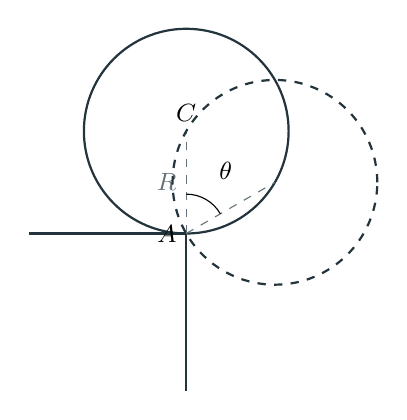
\begin{tikzpicture}[font=\small]
\draw[object](-2,0)--(0,0)--(0,-2);\draw[object](0,1.3)circle(1.3);\draw[guide](0,0)--(0,1.3)node[midway,left]{$R$};\node[left]at(0,0){$A$};\node[above]at(0,1.3){$C$};\draw[guide](0,0)--(1.125833025,.65);\draw[object,dashed](1.125833025,.65)circle(1.3);\draw(0,.5)arc(90:30:.5);\node at(.5,.8){$\theta$};
\end{tikzpicture}
\figcaption{图 6.4\quad 圆心绕固定桌角向右下方移动。}
\end{minipage}\end{center}

\workarea

\clearpage

\pdfbookmark[2]{第 5 题 甲虫落到可转动麦杆后的运动}{q5}

\section*{第 5 题\quad 甲虫落到可转动麦杆后的运动}

\tagline{M-06-05}

如图,均匀细麦杆长\(l\),可绕通过中心\(O\)的固定水平轴在铅垂面内自由转动.开始时麦杆静止于水平位置.一质量与麦杆相同的甲虫以速度\(v_{0}\)垂直落到麦杆的\(\frac{1}{4}\)长度处,落下后立即向端点爬行.

试问:1. 为使麦杆以均匀的角速度转动,甲虫沿麦杆爬行的速度应是多少? 2.
甲虫轨迹的参变方程是什么? 3.
为了使甲虫在麦杆转到铅直位置前能爬到端点,甲虫下落速度 \(v_{0}\)
的最高值是多少?

\begin{center}\begin{minipage}{\linewidth}\centering
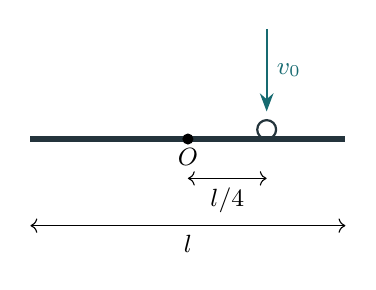
\begin{tikzpicture}[font=\small]
\draw[object,line width=2pt](-2,0)--(2,0);\fill(0,0)circle(2pt)node[below]{$O$};\draw[object](1,.12)circle(.12);\draw[motion](1,1.4)--(1,.35)node[midway,right]{$v_0$};\draw[<->](0,-.5)--(1,-.5)node[midway,below]{$l/4$};\draw[<->](-2,-1.1)--(2,-1.1)node[midway,below]{$l$};
\end{tikzpicture}
\figcaption{图 6.5\quad 甲虫落点离中心 $l/4$，随后沿杆向右端爬行。}
\end{minipage}\end{center}

\workarea

\clearpage

\pdfbookmark[2]{第 6 题 圆柱滚上台阶的速度范围}{q6}

\section*{第 6 题\quad 圆柱滚上台阶的速度范围}

\tagline{M-06-06}

如图6.6,半径为\(R\)的均匀实心圆柱体在水平地面上作纯滚动,其中心\(C\)点的速

度为 \(v_{0}\), 它向前滚动时遇到一个高为 \(h\) 的台阶,
并发出完全非弹性碰撞. 设圆柱和台阶前缘之间的摩擦系数足够大.

试问：1.\(v_{0}\) 为何值时圆柱体能不脱离 A 点而滚上台阶继续前进？2.
对台阶高度 h 有什么限制？

\begin{center}\begin{minipage}{\linewidth}\centering
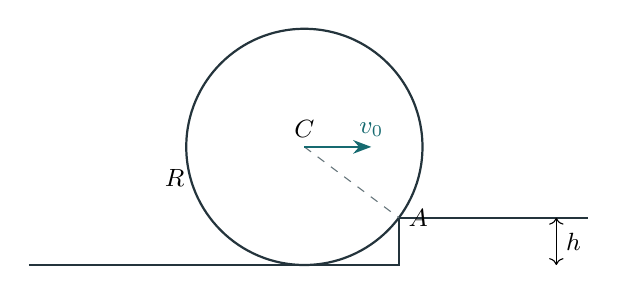
\begin{tikzpicture}[font=\small]
\draw[object](-3.7,0)--(1,0)--(1,.6)--(3.4,.6);\coordinate(A)at(1,.6);\coordinate(C)at(-.2,1.5);\draw[object](C)circle(1.5);\draw[guide](C)--(A);\node[above]at(C){$C$};\node[right]at(A){$A$};\draw[motion](C)--++(.85,0)node[above]{$v_0$};\draw[<->](3,0)--(3,.6)node[midway,right]{$h$};\node[left]at(-1.6,1.1){$R$};
\end{tikzpicture}
\figcaption{图 6.6\quad 碰前仍接地，台阶前缘 $A$ 是碰后上翻的接触点。}
\end{minipage}\end{center}

\workarea

\clearpage

\pdfbookmark[2]{第 7 题 地月系统角动量与月球退行}{q7}

\section*{第 7 题\quad 地月系统角动量与月球退行}

\tagline{M-06-07}

如图,地球和月球的质量分别为\(M_{\mathrm{E}}\)和\(M_{\mathrm{m}}\),两者中心的距离用\(r\)表示,月球可看作质点．设地球的自转轴和月球绕地球作圆周运动的转轴重合，都通过地球中心，地球和月球的角速度分别为
\(\omega_{E}\) 和 \(\omega_{m}\)
．由于潮汐运动，地球自转角速度会发生微小变化，从而地球和月球的间距以及地球和月球系统的总能量也将发生变化．

1.试证明,地球和月球间距的时间变化率 \(\dot{r}\)
与地球自转角速度的时间变化率 \(\dot{\omega}_{\mathrm{E}}\) 的关系为

\[
\dot{ r } = - \frac{ 2 \sqrt{ r } \; I_{ E } } { M_{ \mathrm{m} } \sqrt{ G M_{ E } } } \dot{ \omega }_{ E }
\]

式中 \(I_{\mathrm{E}}\) 是地球对自转轴的转动惯量, \(G\) 是引力常量.

试导出地球和月球系统机械能时间变化率的表达式.

设现在的地球与月球间距为 \(r(0)\), 地球的自转角速度为
\(\omega_{\mathrm{E}}(0)\), 受扰动后相应的量变为 \(r(t)\) 和
\(\omega_{\mathrm{E}}(t)\), 因扰动很小, 月球仍作圆周运动. 试证明

\[
\omega_{ \mathrm{E} } ( t ) = \omega_{ \mathrm{E} } ( 0 ) - \frac{ M_{ \mathrm{m} } \sqrt{ G M_{ \mathrm{E} } } } { I_{ \mathrm{E} } } [ \sqrt{ r ( t ) } - \sqrt{ r ( 0 ) } ]
\]

已知
\(G=6.672 \times 10^{-11} \mathrm{N} \cdot \mathrm{m}^{2} / \mathrm{kg}^{2}, M_{\mathrm{E}}=5.89 \times 10^{24} \mathrm{kg}, M_{\mathrm{m}}=7.34 \times 10^{22} \mathrm{kg}, r=3.84 \times 10^{8} \mathrm{m}\),
\(R_{\mathrm{E}}=6.37 \times 10^{6} \mathrm{m}\) (地球半径).
试计算地球和月球间距增加 2\% 时, 地球日将变成多少小时.

数值计算将地球视为均匀实心球，初始自转周期取 \(24\,\mathrm h\)。

\begin{center}\begin{minipage}{\linewidth}\centering
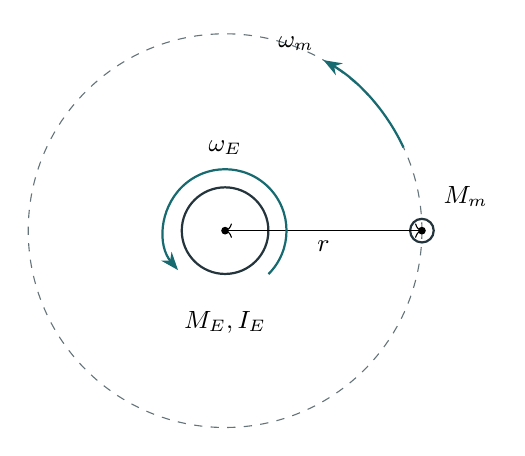
\begin{tikzpicture}[font=\small]
\draw[guide](0,0)circle(2.5);\draw[object](0,0)circle(.55);
\draw[object](2.5,0)circle(.15);\fill(0,0)circle(1.4pt);\fill(2.5,0)circle(1.4pt);
\draw[<->](0,0)--(2.5,0)node[midway,below]{$r$};
\draw[motion](.551543289,-.551543289)arc(-45:220:.78);
\draw[motion](2.265769467,1.056545654)arc(25:60:2.5);
\node[below]at(0,-.9){$M_E,I_E$};
\node[above right]at(2.65,.18){$M_m$};
\node at(0,1.05){$\omega_E$};
\node[above left]at(1.25,2.165063509){$\omega_m$};
\end{tikzpicture}
\figcaption{图 6.7\quad 示意自转与同向圆轨道；图的比例不用于数值计算。}
\end{minipage}\end{center}

\par\vspace{5mm}\noindent{\small\color{muted}作答区}\par\vspace{4mm}\noindent\textcolor{rulegray}{\rule{\linewidth}{0.3pt}}\par\vspace{16mm}\noindent\textcolor{rulegray}{\rule{\linewidth}{0.3pt}}\par\vspace{16mm}\noindent\textcolor{rulegray}{\rule{\linewidth}{0.3pt}}

\clearpage

\pdfbookmark[2]{第 8 题 行星自转与卫星圆轨道的角动量转移}{q8}

\section*{第 8 题\quad 行星自转与卫星圆轨道的角动量转移}

\tagline{M-06-08}

某行星相对其质心轴的转动惯量为 \(I\), 自转角速度为 \(\Omega\). 质量为
\(m\) 的卫星(可看作质点)绕该行星沿圆轨道运动, 轨道半径为 \(r\), 角速度为
\(\omega\), 假定两种角速度的方向一致.

一般情形下 \(\Omega\) 与 \(\omega\) 并不相等, 由于行星上的潮汐摩擦,
行星自转角速度将发生变化, 卫星的圆运动角速度也将相应地改变,
试求两种角速度的改变量之间的关系.

2.潮汐摩擦将引起行星与卫星系统机械能的损耗,试问在什么情形下系统机械能可达稳定值.

\begin{center}\begin{minipage}{\linewidth}\centering
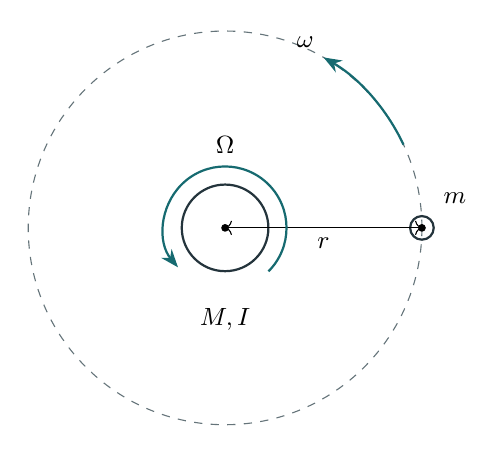
\begin{tikzpicture}[font=\small]
\draw[guide](0,0)circle(2.5);\draw[object](0,0)circle(.55);
\draw[object](2.5,0)circle(.15);\fill(0,0)circle(1.4pt);\fill(2.5,0)circle(1.4pt);
\draw[<->](0,0)--(2.5,0)node[midway,below]{$r$};
\draw[motion](.551543289,-.551543289)arc(-45:220:.78);
\draw[motion](2.265769467,1.056545654)arc(25:60:2.5);
\node[below]at(0,-.9){$M,I$};
\node[above right]at(2.65,.18){$m$};
\node at(0,1.05){$\Omega$};
\node[above left]at(1.25,2.165063509){$\omega$};
\end{tikzpicture}
\figcaption{图 6.8\quad 行星自转与卫星圆轨道之间转移角动量。}
\end{minipage}\end{center}

\workarea

\clearpage

\pdfbookmark[2]{第 9 题 线轴受拉时的滚动方向与加速度}{q9}

\section*{第 9 题\quad 线轴受拉时的滚动方向与加速度}

\tagline{M-06-09}

如图,一线轴质量为\(m\),绕质心轴的转动惯量为\(I\),大小半径分别为\(R\)和\(r\),轴上绕线,

以力 \(F\) 拉线,拉力方向与水平面的夹角用 \(\theta\) 表示.
线轴放置在水平桌面上,与桌面之间的摩擦系数为
\(\mu\),试讨论线轴的运动情况.

\begin{center}\begin{minipage}{\linewidth}\centering
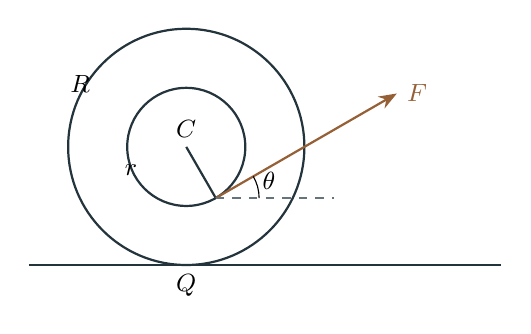
\begin{tikzpicture}[font=\small]
\draw[object](-2,-1.5)--(4,-1.5);\draw[object](0,0)circle(1.5);\draw[object](0,0)circle(.75);\coordinate(P)at(.375,-.649519053);\draw[object](0,0)--(P);\draw[force](P)--++(2.3,1.327905619)node[right]{$F$};\draw[guide](P)--++(1.5,0);\draw (.925,-.649519053)arc(0:30:.55);\node at(1.05,-.43){$\theta$};\node[above]at(0,0){$C$};\node[left]at(-1.1,.8){$R$};\node[left]at(-.5,-.3){$r$};\node[below]at(0,-1.5){$Q$};
\end{tikzpicture}
\figcaption{图 6.9\quad 拉线与内轴下侧相切；$Q$ 为桌面接触点。}
\end{minipage}\end{center}

\workarea

\clearpage

\pdfbookmark[2]{第 10 题 斜面木块牵引实心圆柱体的滚动动力学}{q10}

\section*{第 10 题\quad 斜面木块牵引实心圆柱体的滚动动力学}

\tagline{M-06-10}

如图6.10,在\(\alpha=30^{\circ}\)的斜面上,质量\(m_{2}=4\ \mathrm{kg}\)的木块经轻绳与质量\(m_{1}=8\ \mathrm{kg}\)、半径\(r=5\ \mathrm{cm}\)的实圆柱体的转轴相连.已知斜面的摩擦系数\(\mu=0.2\),圆柱体轴承中的摩擦可以忽略.试求物体的加速度\(a\),并讨论加速度\(a\)、张力\(T\)、圆柱体所受摩擦力\(f_{1}\)随斜面倾角\(\alpha\)的变化.

讨论各倾角时，均取两物体从静止释放，静、动摩擦系数均取题给值。

\begin{center}\begin{minipage}{\linewidth}\centering
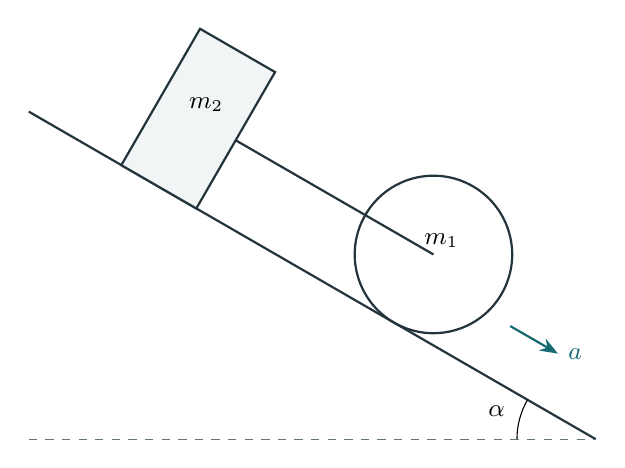
\begin{tikzpicture}[font=\small]
\draw[object](-3.6,2.08)--(3.6,-2.08);\begin{scope}[rotate=-30]\draw[object,fill=rulegray!30](-2.8,0)rectangle(-1.7,2);\draw[object](1.2,1)circle(1);\draw[object](-1.7,1)--(1.2,1);\node at(-2.25,1.2){$m_2$};\node at(1.2,1.2){$m_1$};\draw[motion](2.5,.7)--(3.2,.7)node[right]{$a$};\end{scope}\draw(2.6,-2.08)arc(180:150:1);\node at(2.34,-1.73){$\alpha$};\draw[guide](-3.6,-2.08)--(3.6,-2.08);
\end{tikzpicture}
\figcaption{图 6.10\quad 圆柱在下坡一侧，绳在轴心处牵引。}
\end{minipage}\end{center}

\workarea

\clearpage

\pdfbookmark[2]{第 11 题 逆向自旋乒乓球由滚滑转为纯滚}{q11}

\section*{第 11 题\quad 逆向自旋乒乓球由滚滑转为纯滚}

\tagline{M-06-11}

如图,半径为\(R\)的乒乓球,绕质心轴的转动惯量\(I=\frac{2}{3}mR^{2}\),\(m\)为乒乓球的质量,以一定的初始条件在粗糙的水平面上运动．开始时球的质心速度为
\(v_{\mathrm{C}0}>0\)，向右；初角速度为
\(\omega_0>0\)，逆时针．已知乒乓球与地面之间的摩擦系数为 \(\mu\) .
试求乒乓球开始作纯滚运动所需的时间及纯滚时的质心速度．

\begin{center}\begin{minipage}{\linewidth}\centering
\begin{tikzpicture}[font=\small]
\draw[object](-2,-1)--(3,-1);\draw[object](0,0)circle(1);\draw[motion](0,0)--(1.8,0)node[right]{$v_0$};\draw[motion](.650538239,.650538239)arc(45:250:.92);\node[left]at(-1.2,.5){$\omega_0$ 逆时针};\node[below]at(0,-1){$P$};\node at(.5,-1.9){$I=2mR^2/3$};
\end{tikzpicture}
\figcaption{图 6.11\quad 质心向右、自旋逆时针，最低点起初向右滑。}
\end{minipage}\end{center}

\workarea

\clearpage

\pdfbookmark[2]{第 12 题 圆柱体滚下斜坡撞墙后的回升高度}{q12}

\section*{第 12 题\quad 圆柱体滚下斜坡撞墙后的回升高度}

\tagline{M-06-12}

如图,实心圆柱体从高度为\(h\)的斜坡上从静止纯滚动地到达水平地面上,继续纯滚动,与光滑竖直墙作完全弹性碰撞后返回,经足够长的水平距离后重新作纯滚动,并纯滚动地爬上斜坡.设地面与圆柱体之间的摩擦系数为\(\mu\),试求圆柱体爬坡所能达到的高度\(h'\).

\begin{center}\begin{minipage}{\linewidth}\centering
\begin{tikzpicture}[font=\small]
\draw[object](-4,3.4)--(-4,0)--(1,0)--(3.55,2.55);
\coordinate(Ci)at(2.730761185,2.65);\coordinate(Cb)at(-1,.65);
\draw[object](Ci)circle(.65);\draw[object](Cb)circle(.65);
\draw[motion](Cb)--(-2.2,.65)node[above]{$v_0$};
\node[above]at(Ci){$v=0$};\node[left]at(-4,2.3){光滑墙};
\draw[guide](Ci)--(4.3,2.65);\draw[guide](1,.65)--(4.3,.65);
\draw[<->](4.05,.65)--(4.05,2.65)node[midway,right]{$h$};
\end{tikzpicture}
\figcaption{图 6.12\quad 高度按质心相对水平段质心的位置量取；光滑墙弹性反弹后返回。}
\end{minipage}\end{center}

\workarea

\clearpage

\pdfbookmark[2]{第 13 题 小球沿圆柱面滚下的无滑条件}{q13}

\section*{第 13 题\quad 小球沿圆柱面滚下的无滑条件}

\tagline{M-06-13}

半径为$r$、质量为$m$的均匀实心小球，从半径为$R$的固定圆柱面顶端自静止滚下。
球心位置角$\varphi$从竖直向上方向量起，静、动摩擦系数均取$\mu$。
\begin{enumerate}
\item 为保证$0\leq\varphi\leq45^\circ$内小球纯滚，求$\mu$的最小值。
\item 取$\mu=0.7$，求纯滚结束时的质心速度$v_1$。
\item 求离开圆柱面的位置角$\varphi_2$满足的方程，不必求解。
\end{enumerate}
运动理解为顶端静止经无穷小偏离后的过程。

\begin{center}\begin{minipage}{\linewidth}\centering
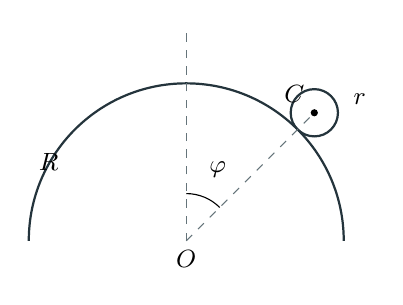
\begin{tikzpicture}[font=\small]
\draw[object](-2,0)arc(180:0:2);
\coordinate(C)at(1.626345597,1.626345597);\coordinate(P)at(1.414213562,1.414213562);
\draw[object](C)circle(.3);\draw[guide](0,0)--(C);
\draw[guide](0,0)--(0,2.7);\draw(0,.6)arc(90:45:.6);
\node at(.4,.9){$\varphi$};\node[below]at(0,0){$O$};
\node[left]at(-1.5,1){$R$};\fill(C)circle(1.3pt);
\node[above left]at(C){$C$};\node[right]at(2,1.8){$r$};
\end{tikzpicture}
\figcaption{图 6.13\quad 小球质心沿半径 $R+r$ 的外侧圆周运动。}
\end{minipage}\end{center}

\workarea

\clearpage

\pdfbookmark[2]{第 14 题 两相同实心球弹性碰撞后的滚动}{q14}

\section*{第 14 题\quad 两相同实心球弹性碰撞后的滚动}

\tagline{M-06-14}

在水平地面上有两个完全相同的均匀实心球,其一作纯滚动,质心速度为\(v\),另一静止不动.两球作完全弹性碰撞,因碰撞时间很短,碰撞过程中摩擦力的影响可以忽略不计.

试求:1. 碰后两球达到纯滚时的质心速度. 2. 全部过程中损失的机械能的百分数.

两球沿连心线正碰，球间无切向冲量；地面粗糙，碰后有充分时间达到纯滚。

\begin{center}\begin{minipage}{\linewidth}\centering
\begin{tikzpicture}[font=\small]
\draw[object](-2,-.7)--(4,-.7);\foreach \x/\s in {0/1,2.4/2}{\draw[object](\x,0)circle(.7);\node at(\x,.1){球\s};}\draw[motion](0,.95)--(1.5,.95)node[right]{$v$};\draw[motion](-.494974747,.494974747)arc(135:-100:.7);\node[below]at(2.4,-1){静止};
\end{tikzpicture}
\figcaption{图 6.14\quad 球1纯滚，沿连心线正碰静止球2。}
\end{minipage}\end{center}

\workarea

\clearpage

\pdfbookmark[2]{第 15 题 两圆柱轮与轻杆连接系统的运动}{q15}

\section*{第 15 题\quad 两圆柱轮与轻杆连接系统的运动}

\tagline{M-06-15}

如图,两个质量和半径均相同的实心圆柱轮,它们的质心轴互相平行,并用一轻杆相

连,轴与轴承间的摩擦忽略不计. 两轮先以共同的初速 \(v_{0}\)
沿水平方向运动,两轮的初角速度为零(如上图).
然后同时轻轻与地面相接触(如下图). 设两轮与地面之间的摩擦系数分别为
\(\mu_{1}\) 和 \(\mu_{2}(\mu_{1}>\mu_{2})\).
试求两轮均变为纯滚动所需的时间及纯滚后的平动速度.

\begin{center}\begin{minipage}{\linewidth}\centering
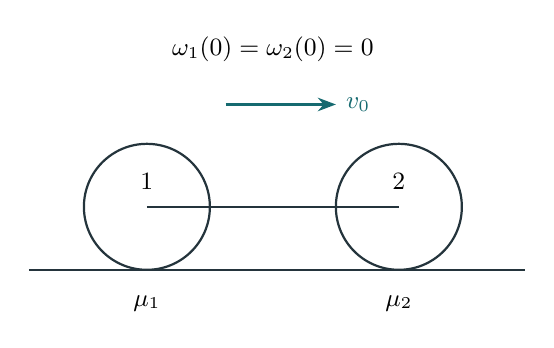
\begin{tikzpicture}[font=\small]
\draw[object](-1.5,-.8)--(4.8,-.8);\foreach \x/\i in {0/1,3.2/2}{\draw[object](\x,0)circle(.8);\node[above]at(\x,.1){\i};\node[below]at(\x,-1){$\mu_\i$};}\draw[object](0,0)--(3.2,0);\draw[motion](1,1.3)--(2.4,1.3)node[right]{$v_0$};\node at(1.6,2){$\omega_1(0)=\omega_2(0)=0$};
\end{tikzpicture}
\figcaption{图 6.15\quad 轻杆连接轴心；两轮角速度可以不同。}
\end{minipage}\end{center}

\workarea

\clearpage

\pdfbookmark[2]{第 16 题 带初始自旋实心球碰地后的反弹}{q16}

\section*{第 16 题\quad 带初始自旋实心球碰地后的反弹}

\tagline{M-06-16}

如图6.16,一半径为\(R\)的实心均匀球,开始时质心静止,但绕通过质心的水平轴以角速度
\(\omega_{0}\) 旋转,在重力作用下垂直下落到地面,球上最低点离地面的高度为
\(h\). 球与地面碰撞的恢复系数为 \(e\),球与地面之间的摩擦系数为
\(\mu\),忽略空气阻力及碰撞时产生的形变.

试求碰地后球的质心速度和自转角速度.

试求第一次落地点与第二次落地点之间的水平距离.

试画出碰后球的质心速度与地面夹角 \(\theta\) 的正切与初始角速度
\(\omega_{0}\) 的关系曲线.

\begin{center}\begin{minipage}{\linewidth}\centering
\begin{tikzpicture}[font=\small]
\draw[object](-2,0)--(2,0);\draw[object](0,2.5)circle(.7);\draw[motion](-.494974747,2.994974747)arc(135:-80:.7);\node[right]at(1,2.5){$\omega_0$};\draw[<->](-1.3,0)--(-1.3,1.8)node[midway,left]{$h$};\draw[motion](0,1.8)--(0,.8);\node[right]at(.2,1.1){自由下落};
\end{tikzpicture}
\figcaption{图 6.16\quad 初态无质心平移，底部自旋方向为向左。}
\end{minipage}\end{center}

\workarea

\clearpage

\pdfbookmark[2]{第 17 题 圆柱体在可动斜面上无滑滚动}{q17}

\section*{第 17 题\quad 圆柱体在可动斜面上无滑滚动}

\tagline{M-06-17}

如图,斜面体放置在光滑水平面上,斜面倾角为\(\theta\),一半径为\(R\)的均匀实心圆柱体在斜面上无滑动地下滚.设斜面体和圆柱体具有相同的质量\(m\),试求斜面体的加速度.

\begin{center}\begin{minipage}{\linewidth}\centering
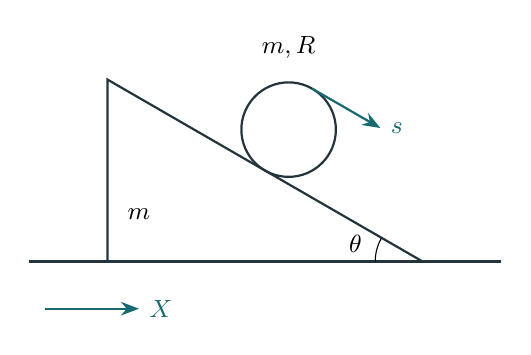
\begin{tikzpicture}[font=\small]
\draw[object](-3,0)--(3,0);\draw[object](-2,2.309401077)--(2,0)--(-2,0)--cycle;
\coordinate(C)at(.3,1.674315780);\draw[object](C)circle(.6);
\node at(-1.6,.6){$m$};\node[above]at(.3,2.45){$m,R$};
\draw[motion](.6,2.193931022)--(1.466025404,1.693931022)node[right]{$s$};
\draw[motion](-2.8,-.6)--(-1.6,-.6)node[right]{$X$};
\draw(1.4,0)arc(180:150:.6);\node at(1.15,.22){$\theta$};
\end{tikzpicture}
\figcaption{图 6.17\quad $s$的正向沿斜面向右下，$X$的正向沿地面向右；圆柱相对斜面无滑动。}
\end{minipage}\end{center}

\workarea

\clearpage

\pdfbookmark[2]{第 18 题 实心球在水平面内的滚滑运动}{q18}

\section*{第 18 题\quad 实心球在水平面内的滚滑运动}

\tagline{M-06-18}

质量为$m$、半径为$r$的均匀实心球在粗糙水平面上运动，
球心$C$的初始水平速度为$\boldsymbol v_0$，
绕球心的初始角速度为任意方向的$\boldsymbol\omega_0$。
球与水平面间摩擦系数为$\mu$，按最低点的库仑滑动摩擦处理。
试分析滚滑过程、转入无滑的时刻与终态，以及质心轨迹。

\begin{center}\begin{minipage}{\linewidth}\centering
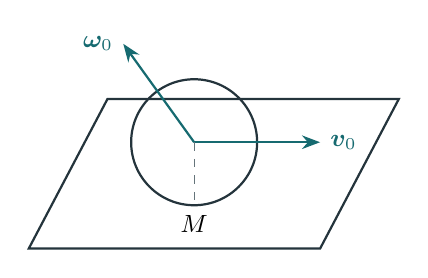
\begin{tikzpicture}[font=\small]
\draw[object](-1.7,-1.2)--(2,-1.2)--(3,.7)--(-.7,.7)--cycle;\draw[object](.4,.15)circle(.8);\draw[motion](.4,.15)--(2,.15)node[right]{$\boldsymbol v_0$};\draw[motion](.4,.15)--(-.5,1.4)node[left]{$\boldsymbol\omega_0$};\draw[guide](.4,.15)--(.4,-.65);\node[below]at(.4,-.65){$M$};
\end{tikzpicture}
\figcaption{图 6.18\quad 球可同时具有任意方向自旋与水平质心速度。}
\end{minipage}\end{center}

\workarea

\clearpage

\pdfbookmark[2]{第 19 题 两均匀圆盘偏心碰撞后的速度与转动}{q19}

\section*{第 19 题\quad 两均匀圆盘偏心碰撞后的速度与转动}

\tagline{M-06-19}

如图6.19,一个质量为\(m\),半径为\(R_A\)的均匀圆盘\(A\)在光滑水平面Oxy内以速度\(V\)沿\(x\)方向平动,圆盘中心至\(x\)轴的垂直距离为\(b\).圆盘\(A\)与另一静止的、其中心位于坐标原点\(O\)的均匀圆盘\(B\)相碰.圆盘\(B\)的质量与\(A\)相同,半径为\(R_B\).假定碰撞后两圆盘接触处的切向速度分量(垂直于连心线方向的速度)相等,并假定碰撞前、后两盘沿连心线方向的相对速度大小不变.在发生碰撞的情况下,试求:

碰后两圆盘质心速度的 \(x\) 分量和 \(y\) 分量 \(V'_{Ax}\), \(V'_{Ay}\),
\(V'_{Bx}\), \(V'_{By}\). 结果要以给定的参数 \(m\), \(R_A\), \(R_B\),
\(V\) 和 \(b\) 表示.

碰后两圆盘的动能 \(E'_A\) 和 \(E'_B\), 结果要以给定的参数 \(m\),
\(R_A\), \(R_B\), \(V\) 和 \(b\) 表示.

\begin{center}\begin{minipage}{\linewidth}\centering
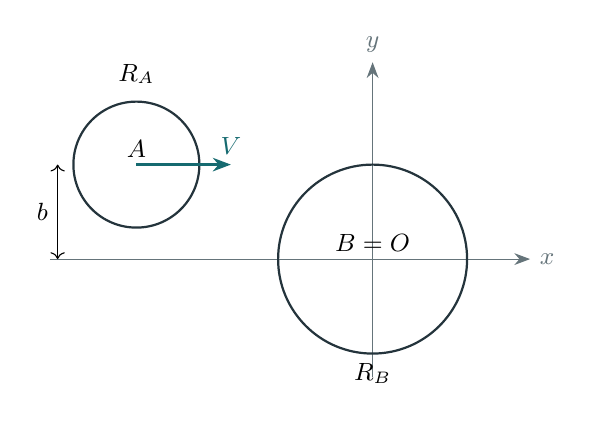
\begin{tikzpicture}[font=\small]
\draw[axis](-4.1,0)--(2,0)node[right]{$x$};\draw[axis](0,-1.5)--(0,2.5)node[above]{$y$};
\draw[object](0,0)circle(1.2);\draw[object](-3,1.2)circle(.8);
\draw[motion](-3,1.2)--(-1.8,1.2)node[above]{$V$};
\draw[<->](-4,0)--(-4,1.2)node[midway,left]{$b$};
\node at(0,.2){$B=O$};\node at(-3,1.4){$A$};
\node[below]at(0,-1.2){$R_B$};\node[above]at(-3,2.1){$R_A$};
\end{tikzpicture}
\figcaption{图 6.19\quad 水平面俯视图；盘A初始无自旋。}
\end{minipage}\end{center}

\workarea

\clearpage

\pdfbookmark[2]{第 20 题 细圆环在粗糙桌面上的滑动与转动衰减}{q20}

\section*{第 20 题\quad 细圆环在粗糙桌面上的滑动与转动衰减}

\tagline{M-06-20}

如图6.20,均匀细圆环半径为\(R\),质量为\(m\),平放在水平桌面上,与桌面之间的摩擦系数为\(\mu\).圆环质心\(O\)沿\(x\)轴以初速\(v_{\mathrm{C}0}\)运动,同时圆环绕质心以初角速度\(\omega_{0}\)顺时针转动,\(v_{\mathrm{C}0}\)与\(\omega_{0}\)满足\(v_{\mathrm{C}0}=R\omega_{0}\).

试求:1. 圆环所受摩擦力及摩擦力对质心的力矩. 2.
从开始到圆环停止运动所需时间.

\begin{center}\begin{minipage}{\linewidth}\centering
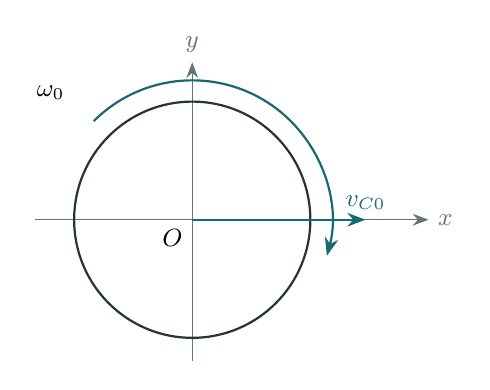
\begin{tikzpicture}[font=\small]
\draw[axis](-2,0)--(3,0)node[right]{$x$};\draw[axis](0,-1.8)--(0,2)node[above]{$y$};\draw[object](0,0)circle(1.5);\draw[motion](0,0)--(2.2,0)node[above]{$v_{C0}$};\draw[motion](-1.251579003,1.251579003)arc(135:-15:1.77);\node[above left]at(-1.5,1.4){$\omega_0$};\node[below left]at(0,0){$O$};
\end{tikzpicture}
\figcaption{图 6.20\quad 圆环平放桌面，题给 $v_{C0}=R\omega_0$。}
\end{minipage}\end{center}

\workarea

\clearpage

\pdfbookmark[2]{第 21 题 竖直均匀细杆在光滑地面上倒下}{q21}

\section*{第 21 题\quad 竖直均匀细杆在光滑地面上倒下}

\tagline{M-06-21}

长为\(l\)的均匀细杆竖直地放置在光滑地面上,从静止倒下．试求落到地面时的质心速度．

初态从静止作无穷小偏离后开始运动。

\begin{center}\begin{minipage}{\linewidth}\centering
\begin{tikzpicture}[font=\small]
\draw[object](-2.2,0)--(2.2,0);
\draw[object,line width=2pt](0,0)--(0,3.6);
\draw[object,dashed,line width=1.3pt](-1.157017697,0)--(1.157017697,2.757759995);
\draw[guide](0,0)--(0,3.9);
\fill(0,1.378879998)circle(1.5pt)node[left]{$C$};
\node[right]at(.15,3.25){$l$};\node[below]at(-1.157017697,0){$B$};
\node[right]at(1.157017697,2.757759995){$A$};
\draw[motion](-.3,-.45)--(-1.3,-.45)node[midway,below]{下端左移};
\end{tikzpicture}
\figcaption{图 6.21\quad 倒下时质心水平位置不变，下端向左滑动。}
\end{minipage}\end{center}

\workarea

\clearpage

\pdfbookmark[2]{第 22 题 质点撞击光滑地面上均匀细杆}{q22}

\section*{第 22 题\quad 质点撞击光滑地面上均匀细杆}

\tagline{M-06-22}

如图6.22,光滑水平地面上静止地放着质量为 \(M\) 、长为 \(l\) 的均匀细杆.
质量为 \(m\) 的质点以垂直于杆的水平初速 \(v_0\) 与杆的一端作完

全非弹性碰撞.

试求:1. 碰后系统质心的速度及绕质心的角速度. 2.
实际的转轴(即静止点)位于何处.

\begin{center}\begin{minipage}{\linewidth}\centering
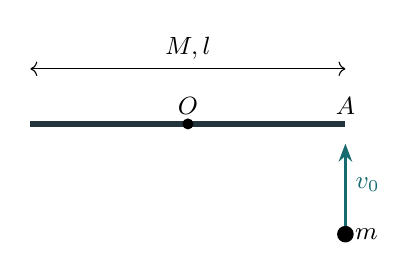
\begin{tikzpicture}[font=\small]
\draw[object,line width=2pt](-2,0)--(2,0);\fill(0,0)circle(2pt)node[above]{$O$};\fill(2,-1.4)circle(3pt)node[right]{$m$};\draw[motion](2,-1.3)--(2,-.25)node[midway,right]{$v_0$};\node[above]at(2,0){$A$};\draw[<->](-2,.7)--(2,.7)node[midway,above]{$M,l$};
\end{tikzpicture}
\figcaption{图 6.22\quad 光滑水平面俯视图；质点撞杆端并粘住。}
\end{minipage}\end{center}

\workarea

\clearpage

\pdfbookmark[2]{第 23 题 细杆靠墙下滑的运动与离墙}{q23}

\section*{第 23 题\quad 细杆靠墙下滑的运动与离墙}

\tagline{M-06-23}

如图,长为 \(2l\)
的均匀细杆,下端支在地面上,上端靠在竖直墙上,从静止下滑,开始时

杆与地面的夹角为 \(\theta_{0}\) . 设杆与地和墙之间的摩擦可略 .
试问质心下降到初始高度的几分之几时,杆的上端与墙脱离 .

\begin{center}\begin{minipage}{\linewidth}\centering
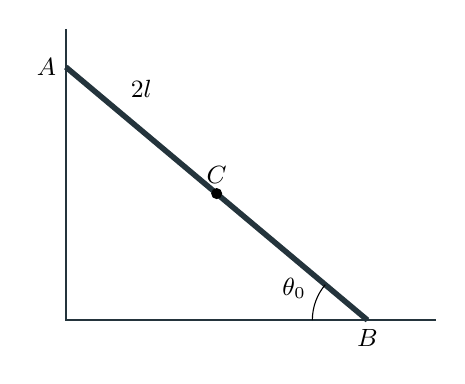
\begin{tikzpicture}[font=\small]
\draw[object](0,3.7)--(0,0)--(4.7,0);\coordinate(A)at(0,3.213938048);\coordinate(B)at(3.830222216,0);\coordinate(C)at(1.915111108,1.606969024);\draw[object,line width=2pt](A)--(B);\fill(C)circle(2pt)node[above]{$C$};\node[left]at(A){$A$};\node[below]at(B){$B$};\draw(3.130222216,0)arc(180:140:.7);\node at(2.9,.4){$\theta_0$};\node[above right]at(.7,2.7){$2l$};
\end{tikzpicture}
\figcaption{图 6.23\quad 两端接触均光滑，初始角为 $\theta_0$。}
\end{minipage}\end{center}

\workarea

\clearpage

\pdfbookmark[2]{第 24 题 单杆与铰接双段杆受相同冲量的动能比较}{q24}

\section*{第 24 题\quad 单杆与铰接双段杆受相同冲量的动能比较}

\tagline{M-06-24}

如图6.24,在光滑地面上静止地放置着两根质量均为 \(m\),长度均为 \(l\)
的均匀细杆.其中一杆由相等的两段构成,中间用光滑的铰链连接起来(意即两段在连接点可以弯折但不能分离).在两杆的一端,各施以相同的垂直于杆的水平冲量
\(J\).试求两杆所获动能之比.

\begin{center}\begin{minipage}{\linewidth}\centering
\begin{tikzpicture}[font=\small]
\draw[object,line width=2pt](-2,1)--(2,1);\draw[object,line width=2pt](-2,-1)--(2,-1);\draw[object,fill=white](0,-1)circle(.12);\foreach \y in {1,-1}{\draw[force](-2,\y-1)--(-2,\y-.1)node[midway,left]{$J$};}\node[right]at(2,1){单杆};\node[right]at(2,-1){两段铰接};
\end{tikzpicture}
\figcaption{图 6.24\quad 两杆总质量、总长度与端部冲量相同。}
\end{minipage}\end{center}

\workarea

\clearpage

\pdfbookmark[2]{第 25 题 旋转圆环中滑动细杆的平衡与稳定性}{q25}

\section*{第 25 题\quad 旋转圆环中滑动细杆的平衡与稳定性}

\tagline{M-06-25}

如图6.25,半径为\(R\)的圆环绕铅垂的直径轴以角速度\(\omega\)匀角速旋转.一细杆长\(L=\sqrt{2}R\),其两端约束在圆环上可作无摩擦滑动,细杆的位置用\(OC\)与铅垂轴的夹角\(\theta\)表示,\(C\)为细杆的质心.试求细杆在圆环上的平衡位置,并讨论平衡的稳定性.

\begin{center}\begin{minipage}{\linewidth}\centering
\begin{tikzpicture}[font=\small]
\draw[object](0,0)circle(2);\draw[axis](0,-2.5)--(0,2.5)node[above]{铅垂轴};\coordinate(C)at(.707106781,-1.224744871);\coordinate(A)at(-.517638090,-1.931851653);\coordinate(B)at(1.931851653,-.517638090);\draw[object,line width=2pt](A)--(B);\draw[guide](0,0)--(C);\fill(C)circle(2pt)node[right]{$C$};\node[above left]at(0,0){$O$};\draw(0,-.7)arc(-90:-60:.7);\node at(.35,-.65){$\theta$};\node[left]at(A){$A$};\node[right]at(B){$B$};
\end{tikzpicture}
\figcaption{图 6.25\quad 杆为圆环的一条弦，$OC$ 垂直杆，角度从向下竖直量起。}
\end{minipage}\end{center}

\workarea

\clearpage

\pdfbookmark[2]{第 26 题 旋转支架上细杆的有效势能与平衡}{q26}

\section*{第 26 题\quad 旋转支架上细杆的有效势能与平衡}

\tagline{M-06-26}

如图, \(Ox\) 和 \(Oy\) 分别是支架的水平臂和铅垂臂, \(Ox\)
臂绕铅垂臂作匀角速转动, 角速度

为 \(\omega\)
.一均匀细杆的两端A和B被分别约束在两臂上运动.假定约束是理想的(即不计摩擦力),细杆的质量为\(m\),长为2L,细杆位置用图中\(\theta\)角表示,\(\theta\)角是OC与Oy之间的夹角,\(C\)为细杆质心.以支架为参考系考察细杆的运动.1.试写出细杆的能量表达式.2.试求细杆的平衡位置,并讨论平衡的稳定性.

\begin{center}\begin{minipage}{\linewidth}\centering
\begin{tikzpicture}[font=\small]
\draw[axis](0,0)--(4.2,0)node[right]{$x$};\draw[axis](0,.8)--(0,-3.8)node[below]{铅垂臂};\coordinate(A)at(0,-2.828427125);\coordinate(B)at(2.828427125,0);\coordinate(C)at(1.414213562,-1.414213562);\draw[object,line width=2pt](A)--(B);\draw[guide](0,0)--(C);\fill(C)circle(2pt)node[right]{$C$};\node[above left]at(0,0){$O$};\node[left]at(A){$A$};\node[above]at(B){$B$};\draw(0,-.7)arc(-90:-45:.7);\node at(.45,-.75){$\theta$};\node[right]at(2,-1.2){$2L$};
\end{tikzpicture}
\figcaption{图 6.26\quad 铅垂臂向下，水平臂绕它转动；$O$ 不在杆上。}
\end{minipage}\end{center}

\workarea

\clearpage

\pdfbookmark[2]{第 27 题 陀螺进动与翻转陀螺的摩擦力矩机制}{q27}

\section*{第 27 题\quad 陀螺进动与翻转陀螺的摩擦力矩机制}

\tagline{M-06-27}

\begin{enumerate}
\def\labelenumi{\arabic{enumi}.}
\tightlist
\item
  如图6.27, 质量为 \(m\) 的陀螺绕对称轴高速旋转, 角速度为 \(\omega\),
  绕对称轴的转动惯量为 \(I\), 质心到转轴下端的距离为 \(l_{\mathrm{C}}\),
  在重力矩的作用下, 陀螺将绕竖直轴作缓慢进动. 试求进动角速度的近似值.
\end{enumerate}

2.若转轴下端与桌面是面接触,并受摩擦力的作用.试解释在摩擦的作用下,转轴将产生趋向于竖直轴的附加运动,并计算从倾斜\(\theta\)角到竖直位置所需的时间.

第二问采用近似模型：接触摩擦的合力 \(f=\mu mg\)，关于质心的有效力臂取
\(l_{\mathrm C}\)，自旋角动量 \(I\omega\) 在扶正过程中近似不变。

\begin{center}\begin{minipage}{\linewidth}\centering
\begin{tikzpicture}[font=\small]
\draw[object](-2,0)--(2,0);\draw[axis](0,0)--(0,3.6)node[above]{竖直};\draw[object,line width=1.7pt](0,0)--(1.3,3);\begin{scope}[shift={(.78,1.8)},rotate=-23.428692809]\draw[object,fill=rulegray!30](-.7,-.25)rectangle(.7,.25);\end{scope}\fill(.78,1.8)circle(2pt)node[right]{$C$};\node[below left]at(0,0){$O$};\draw(0,.7)arc(90:66.571307191:.7);\node at(.35,.9){$\theta$};\draw[motion](.78,1.8)--(1.43,3.3)node[right]{$\boldsymbol L$};
\end{tikzpicture}
\figcaption{图 6.27\quad 高速自旋陀螺；轴向角动量近似占主导。}
\end{minipage}\end{center}

\workarea

\end{document}
